%%%%%%%%%%%%%%%%%%%%%%%%%%%%%%%%%%%%%%%%%%%%%%%%%%%%%%%%%%%%%%%%%%%%%%%%%%%%%%%
% Chapter 4 : Desarrollo y tecnologías utilizadas
%%%%%%%%%%%%%%%%%%%%%%%%%%%%%%%%%%%%%%%%%%%%%%%%%%%%%%%%%%%%%%%%%%%%%%%%%%%%%%%



%++++++++++++++++++++++++++++++++++++++++++++++++++++++++++++++++++++++++++++++

En este capítulo se describirá en profundidad el framework \textbf{genetics.js}. Se expondrán tanto las tecnologías utilizadas, justificando debidamente la elección, así como la propia estructura que tiene el software que se ha desarrollado.

%---------------------------------------------------------------------------------
\section{Tecnologías utilizadas}
\label{4:sec:1}

Dado que el objetivo fundamental de este proyecto es el desarrollo de un framework de computación evolutiva que sea completamente compatible con la web, las tecnologías más apropiadas para este desarrollo serán las que se utilicen en el \textit{stack} del lenguaje JavaScript. \\

Por ello, en primer lugar llevaremos a cabo una introducción a dicho lenguaje de programación, para luego exponer las dependecias externas que se ha utilizado durante la fase de desarrollo y las que se han elegido para ser utilizadas en la versión de la librería en producción, es decir las que serán utilizadas por los usuarios finales. 

\subsection{\textit{Stack} de desarrollo en JavaScript}

En primer lugar, es importante introducir el lenguaje de programación JavaScript y la importancia que tiene hoy en día, exponiendo las tecnologías más comunes que tiene aparejadas el desarrollo de una aplicación con este lenguaje. \\

JavaScript es un lenguaje de programación interpretado, multiparadigma y de tipado débil, desarrollado por Brendan Eich, durante su trabajo en Netscape, para ser utilizado por el navegador que la empresa estaba creando. Durante esa época y en sus primeros años, se consideraba un lenguaje menor, es decir que solo se utilizaba para implementar ciertos aspectos de la interacción del usuario con la página web, o para llevar a cabo operaciones sencillas en el lado del cliente. \\

Debido a la poca importancia que se le dio a su desarrollo desde el momento inicial, son destacables los grandes errores de diseño con los cuales cuenta \cite{KennethEng2019}, y los que hacen que sea bastante complejo confiar en que el software desarrollado en esta tecnología cumplirá ciertos criterios de calidad. Es por ello que diversas empresas e instituciones, han tratado de estandarizar y complementar el lenguaje para garantizar su estabilidad y escalabilidad. Ejemplo de ello, es la organización ECMA con los estándares de JavaScript \cite{ecmascript}, o Microsoft con la creación del lenguaje TypeScript.\\

Con los años ha ganado bastante popularidad, gracias en parte a proyectos como NodeJS \cite{node}, el cual trata de convertir a JavaScript en un lenguaje con mucho más ámbito que el que tenía anteriormente, dando la posibilidad de construir un servidor completo con este lenguaje. NodeJS es una de las tecnologías más punteras para el desarrollo de servidores hoy en día, debido a su gran escalabilidad y a que soporta una gran cantidad de conexiones simultáneas, en parte grecias al uso del motor V8 de JavaScript \cite{motor-v8}, desarrollado por Google. \\

En este sentido, es muy destacable también NPM (Node Package Manager) \cite{npm} como gestor de dependencias de NodeJS. Este gestor de paquetes es el ejemplo perfecto de sencillez y eficacia, al permitir publicar nuestros propios módulos en un portal que los aglutina de manera centralizada, y que nos permite instalar, gestionar y utilizar dichos paquetes de manera sencilla en nuestra propia aplicación desde la línea de comandos. \\

La gestión de dependencias es una tarea compleja que puede acarrear ciertos problemas, sobretodo de retrocompatibilidad entre versiones. Una de las grandes ventajas de NPM es que esta tarea es bastante sencilla, centralizando todas las dependecias en un fichero \textit{json} (\textit{package.json}), en el cual se especifica el nombre del paquete y la versión que tenemos instalada. De esta forma se garantiza que se está utilizando en nuestra aplicación exactamente la dependencia que queremos. \\

Además, el versionado de los paquetes se basa en \textbf{semantic versioning} \cite{semver}, contando con la posibilidad de distinguir entre versiones \textbf{minor, major y patch}, garantizando así que se pueda seguir el mapa de desarrollo previsto. \\

De esta forma, teniendo el potencial de una herramienta como NPM, la posibilidad de llevar esta idea a aplicaciones cliente es bastante interesante, puesto que para la web la importación de módulos externos no se gestiona de una manera tan eficaz que como se hace con NodeJS y NPM. Es ahí donde entran herramientas como Webpack \cite{webpack} y Babel \cite{babel} en juego, las cuales permiten que el código que se importa mediante NPM y se utiliza en ficheros de código fuente, sea compilado para ser utilizado directamente en el \textit{front-end}. De esta forma podemos utilizar NPM como gestor de dependencias aunque estemos trabajando en el lado del cliente. \\

Como vemos, la existencia de este tipo de tecnologías hace que sea muy conveniente desarrollar la librería \textbf{genetics.js} como un módulo NPM, puesto que ya no solo podría ser utillizada en el lado del cliente, sino que también hace posible que se utilice en otros ámbitos como un servidor con NodeJS o cualquier otra tecnología basada en JavaScript.

\subsection{Tecnologías utilizadas para el desarrollo}

Tal y como se ha comentado, la librería \textbf{genetics.js} se desarrollará como un módulo NPM para garantizar que sea compatible con tecnologías web. En este primer apartado, expondremos cuales seran las dependencias que este módulo tendrá en el desarrollo. Estas dependencias realmente no afectarán al usuario final, puesto que no serán descargadas ni utilizadas cuando se instale el paquete, ya que solo son útiles para garantizar y facilitar el desarrollo correcto de la librería. \\

Las tecnologías que se han utilizado como dependencias de desarrollo han sido las siguientes:

\subsubsection{Control de versiones (Git y GitHub)}

Los sistemas de control de versiones sirven para que se pueda llevar un desarrollo organizado del proyecto. Tener un sistema de control de versiones es esencial porque en el repositorio que se cree estará alojado todo el código fuente que se escriba, además del historial de \textit{commits} o confirmaciones que se lleven a cabo, de tal forma que se pueda regresar con facilidad a casi cualquier punto del desarrollo. \\

En este proyecto, he utilizado Git \cite{git} como sistema de control de versiones y GitHub \cite{github} para alojar el repositorio remoto. Además el desarrollo se ha estructurado por ramas, de tal forma que solo se encuentre en \textit{master} la versión estable del proyecto. \\

Para estructurar las ramas he utilizado un convenio de nombres, de tal forma que el desarrollo del contenido de la versión concreta sea el nombre de la rama. Por ejemplo si se está desarrollando la versión 0.1.0, la rama de desarrollo llevará el nombre \textit{v0.1.0-dev}

\subsubsection{TypeScript}
 
 Mas que una dependencia de desarollo, TypeScript es el lenguaje de programación en el que se ha implementado el proyecto. Realmente, se considera una dependencia externa, pues aunque el desarrollo completo se llevado a cabo con este lenguaje, se necesita un compilador a JavaScript para publicar el paquete en NPM, con lo cual el usuario final tan solo utilizará código fuente JavaScript, además de las definiciones de tipos generadas. \\
 
 La utilización de TypeScript como lenguaje de desarrollo viene motivada por las carencias que presenta JavaScript para realizar una librería escalable y con las garantías de calidad que se requieren para que sea fácilmente extensible. \\
 
 TypeScript fue desarrollado por Microsoft y actualmente, su compilador principal es un proyecto de software libre mantenido por la propia empresa bajo la licencia Apache 2.0 \cite{typescriptrepo}. Se trata de un superconjunto de JavaScript, de tal forma que cualquier fichero en JavaScript, también está en TypeScript. Esto tiene como ventaja principal la facilidad de migración de un proyecto en un lenguaje a otro. \\
 
 Las ventaja principal que presenta TypeScript frente a JavaScript es que se trata de un lenguaje con tipos. Las definiciones de tipos hacen que sea más complejo programar con este lenguaje, pero a la vez garantizan mucha más seguridad en el código que se desarrolla, asegurando así que se pueda escalar de una manera mucho más efectiva. \\
 
 Es destacable también, las características que presenta TypeScript que son comunes en los lenguajes orientados a objetos tradicionales; como clases o interfaces, que de manera nativa no son soportadas por JavaScript. Estas características son las idóneas para estructurar el software evitando repeticiones necesarias e imponiendo las estructura que se seguirá en un futuro. \\
 
 Cabe destacar que las opciones del compilador son fácilmente configurables mediante un fichero \textit{json} (\textit{tsconfig.json}). En él se puede especificar multitud de opciones, sin embargo la más relevante es el estándard de JavaScript al que se quiere compilar el proyecto. En el caso de \textbf{genetics.js}, se ha elegido la versión ECMAScript5 puesto que es la que tiene un soporte más amplio por la mayoría de navegadores.
 
\subsubsection{Jest y ts-jest}
 
 Una parte muy importante del desarrollo del software son los tests. Mas aun cuando se trata de una librería en la que van a existir una gran cantidad de clases y estructuras de datos diferentes, en cuyo caso, es muy importante que se desarrolle una batería de tests que garantice su correcto funcionamiento. \\
 
 La tecnología utilizada para este propósito ha sido Jest \cite{jest}, pues nos ofrece múltiples ventajas a la hora de crear test unitarios y parametrizados a medida del componente que estemos comprobando y también porque nos permite realizar de manera sencilla \textit{mockups}, o simulaciones, de resultados de las funciones que queramos testear. \\
 
 El hecho de realizar \textit{mockups} es de gran ventaja en una aplicación como esta, en la que tanta lógica depende de resultados aleatorios. Con esta librería de testing se puede especificar \textit{ad-hoc} cual es el resultado "\textit{aleatorio}" que nos devolverá el generador sin tocar su código fuente y de esta forma, aumentar la robostez de los test, comprobando la lógica del componente externalizándola de los valores aleatorios que le puedan llegar como entrada. \\
 
 Una desventaja de este framework de desarrollo, es que no es completamente compatible con TypeScript en su versión actual, lo cual genera algunos problemas de a la hora de comprobar los tipos de los módulos que se están testeando. A su vez, esto genera algunas incompatibilidades de tipos en cuanto a generar los \textit{mockups}, probablemente porque estos internamente se basen en el tipado débil que presenta el lenguaje JavaScript. Para solucionar estos problemas se recurre a la librería externa \textbf{ts-jest} \cite{tsjest}. \\
 
 Al igual que todas las herramientas utilizadas, Jest tiene también su fichero de configuración (\textit{jestconfig.json}). En el se ha especificado cual será el directorio en el que se almacenarán los test además de indicar que se utilizará \textbf{ts-jest} para procesar aquellos que estén en TypeScript.
 
 \subsubsection{CircleCI}
 
 El paso siguiente después de haber realizado una batería de tests es garantizar que estos se ejecuten de manera continua. Esto quiere decir que sean ejecutados cuando se haga un nuevo \textit{commit} al respositorio remoto. \\
 
 La betería de tests es ejecutada por un servidor externo, lo que también sirve para separar dichos test de nuestra máquina local de desarrollo y comprobar de esta forma si nuestro sistema operativo o alguna configuración local está afectando al funcionamiento del proyecto. \\
 
 Llevar a cabo un procedimiento de integración continua es muy importante para garantizar que si se hace un cambio en una parte concreta de la librería, esto no tiene efectos colaterales en otros módulos. La importancia de esto radica principalemnte en la seguridad que tenemos al añadir nuevas funcionalidades a lo que ya tenemos hecho, de tal forma que incorporar a nuevos colaboradores y aceptar sus cambios no sería tan arriesgado como si tan solo se pasaran los test en local.\\
 
 Para llevar a cabo la integración continua se ha elegido la tecnología \textbf{CircleCI}, aunque hay algunas otras opciones que presentan las mismas características, como por ejemplo, \textbf{TravisCI} \cite{travis}. El fichero de configuración de esta herramienta (\textit{.circleci/config.yml}), es básicamente calcado del estándard utilizado para aplicaciones con NodeJS. En él, tan solo es necesario especificar el comando npm que se utilizará para ejecutar los tests de integración contínua.
 
 \subsubsection{Coveralls}
 
 Otro de los aspectos fundamentales relacionados con los tests es el cubrimiento de código, el \textit{coverage}. El cubrimiento de código es un informe que se genera para especificar el porcentaje de líneas de código que hemos cubierto con nuestros tests. \\
 
 Esta no es una medida infalible del correcto funcionamiento del software desarrollado, sin embargo si que nos da una medida bastante fiable de lo extensos que hemos sido con nuestros tests, mostrando si hemos conseguido cubrir la mayoría de líneas de código existentes en el proyecto.\\
 
 La herramienta encargada de recoger los informes de coverge a partir de los tests utilizados para la integración continua ha sido Coveralls \cite{coveralls}. Para ello, se ha especificado un comando de test ejecutado por la integración continua que garantiza que en el caso de que dichos tests se ejecuten sin errores, se envíe un informe al servidor de coveralls. \\
 
 La configuración de este servicio es bastante simple, pues tan solo habría que especificar en el fichero de configuración (\textit{coveralls.yml}) cual es la herramienta de integración continua que se ha utilizado, en este caso CircleCI.
 
 \subsubsection{TypeDoc}
 
 La documentación es una parte esencial del desarrollo, puesto que facilita la tarea de que los usuarios puedan utilizar los diferentes módulos de la librería, teniendo información de cual será el resultado y los parámetros que se espera cada una de las funciones y cual es el objetivo de las clases desarrolladas. \\
 
 Para elaborar una documentación para nuestro proyecto se ha utilizado \textbf{TypeDoc} \cite{typedoc}. Esta herramienta nos permite hacer comentarios en las clases, métododos, interfaces y variables para luego generar una documentación en formato HTML que puede ser desplegada en GitHub pages. \\
 
 La sintaxis de los comentarios es bastante común, puesto que es muy similar a la que utilizan otras herramientas similares como Doxigen o Javadoc, para lenguajes como C++ y Java. Además, se puede formatear los comentarios, pues también admite sintaxis Markdown.
 
 \subsubsection{TSLint y Prettier}
 
 Para finalizar, expondré estas dos herramientas utilizadas básicamente para formatear el código que se programa, de tal forma que se garantice que sea cual sea el editor y el desarrollador que se incorpore al proyecto, el formato y estándard que se seguirá en el código fuente va a ser el mismo. \\
 
 La herramienta Prettier \cite{prettier} se encarga de hacer este formateo del código. Se configura mediante un fichero (\textit{.prettierrc}), en el que se indican las opciones que se desean cumplir para el código fuente generado. \\
 
 De manera complementaria, la herramienta TSLint \cite{tslint} señala en el editor de código errores tanto sintácticos como de estilo. Se puede por tanto indicar cual será el estándard que queremos que siga nuestro proyecto de software. Existen muchos, aunque uno de los más restrictivos es el diseñado por Airbnb \cite{airbnbjs}. \\
 
 La manera más cómoda para utilizar estas dos herramientas es de manera conjunta con el IDE o editor de código, de tal forma que cuando se almacenen los cambios en un fichero este se formatee de manera automática. En este proyecto se ha utilizado WebStorm \cite{webstorm} como IDE de desarrollo, pero hay otras buenas opciones para este propósito, como Visual Studio Code \cite{vscode} o Atom \cite{atom}.

\subsection{Tecnologías utilizadas en producción}

Las dependencias o tecnologías utilizadas en producción son aquellas que serán usadas por el usuario final cuando instale la librería, y no solo serán útiles durante la fase de desarrollo. \\

En este sentido, se ha tratado de construir una librería \textit{minimalista} en cuanto a dependencias, de tal forma que el paquete incluya las menos posibles en su versión de producción. En una librería de las características de este proyecto, realmente esta tarea es bastante sencilla de llevar a cabo, pues prácticamente todo el trabajo de desarrollo se puede hacer desde cero y sin dependencias externas.\\

De esta forma, tan solo se ha utilizado una dependencia en producción:

\subsubsection{random.js}

Una de las problemáticas de trabajar con un lenguaje como JavaScript es que no existe un módulo de generación de números aletorios realmente efectivo, al estilo de la librería \textbf{random} de C++ \cite{randomcpp}. Además, también se añade la problemática de que al estar trabajando con TypeScript, sería muy conveniente llevar a cabo la comprobación de tipos cuando utilicemos dicho paquete. Debido a estos problemas, la única librería que satisfacía las condiciones de ser un generador de números aleatoios correcto estadísticamente y que trabajara con TypeScript es \textbf{random.js} \cite{randomjs}. \\

La ventaja principal que tiene trabajar con esta librería es que se puede especificar el \textit{engine} y la semilla que se utilizará para generar el número aleatorio. Y cuenta ya con una serie de \textit{engines} predeterminados para generar números aleatorios aprovechando característica concretas del entorno en el que se está ejecutando, como por ejemplo NodeJS o un navegador. \\

Aparte de las ventajas que tiene a la hora de especificar el origen del número aleatorio, es destacable también la facilidad que posee para generar datos de un cierto tipo, como por ejemplo: enteros y flotantes en un rango o valores de verdadero y falso (\textit{boolean}). \\

\begin{lstlisting} [style=JavaScript]
import { bool, MersenneTwister19937 } from 'random-js';

/**
* Genera un bool con un 0.3 de probabilidad
* de ser true.
*/
bool(0.3)(MersenneTwister19937.autoSeed());
\end{lstlisting}

%---------------------------------------------------------------------------------
\section{Estructura del software}
\label{4:sec:2}

En esta sección se describirá cual es la estructura lógica de \textbf{genetics.js}, exponiendo cada una de sus partes y justificando cuáles han sido las decisiones de diseño que se han tomado para su desarrollo.

\subsection{Visión general}

Para construir una librería de algoritmos evolutivos, lo fundamental es que sea capaz de cubrir la mayor parte de operaciones disponibles, y además ofrezca la posibilidad de ser extendida de la manera más cómoda posible. \\

Para ello, el diseño que se ha decidido es una estructura de clases e interfaces a implementar por cada una de las partes fundamentales o componentes de esta librería.

\subsection{Individuos}

Dentro de los algoritmos evolutivos, los individuos son quizás la parte fundamental. La idea principal de su diseño para esta librería es la de simplificar lo máximo posible las tareas de evaluación y modificación de su contenido. \\

En computación evolutiva, los individuos codifican una solución concreta de un problema. Este individuo contendrá una serie de datos, que se conocen como el \textbf{genotipo} o codificación de dicha solución. A partir de este genotipo, se puede extraer la información que verdaderamente sería la solución a nuestro problema y que se conoce como \textbf{fenotipo}. \\

Para llevar a cabo la conversión entre genotipo y fenotipo, se debe disponer de la información concreta del problema, y por tanto tener una función que converta el genotipo de un individuo a una solución concreta del espacio de soluciones. \\

Un ejemplo de esto podría ser un problema en el que se quiere buscar el máximo de una función en un dominio de números enteros. Una posible codificación puede ser establecer una correspondencia entre cada uno de los enteros presentes en el dominio y un individuo formado por una cadena de números binarios. Cuando se desee evaular un individuo, lo que se debe hacer es decodificar el número entero al que se corresponde la cadena binaria que contiene dicho individuo. \\

Elegir una buena codificación para nuestro problema es una tarea muy importante y en ocasiones compleja, puesto que la calidad del algoritmo que se diseñe en gran medida dependerá de esta decisión. Además, es importante destacar que dependiendo de la codificación que hayamos elegido, se le podrán aplicar a los individuos involucrados en el algoritmo unas operaciones u otras. \\

Tal y como se ha comentado, la representación de los individuos es casi infinita, pues depende mucho del dominio del problema que se esté tratando de resolver. En \textbf{genetics.js} la decisión que se ha tomado es implementar una jerarquía de clases para modelar esta realidad. \\

En este diagrama UML se puede ver la estructura de clases elegida, de las cuales será necesario explicar cada una de sus partes.

\subsubsection{BaseIndividual}

\begin{figure}[ht]
    \centering
    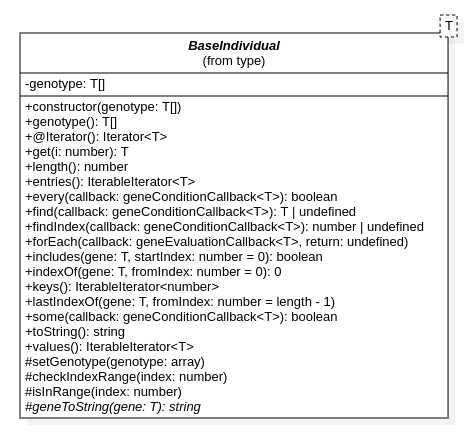
\includegraphics[scale=0.6]{mem/images/cap-4/4.2.2(Individuos)/BaseIndividual.png}
    \caption{Diagrama de clase de \texttt{BaseIndividual}}
    \label{fig:baseindividual-uml}
\end{figure}

\texttt{BaseIndividual} es una clase abstracta que representa al individuo base de la jerarquía. En ella se almacena el \texttt{array} que contiene el genotipo del individuo.
Cabe destacar que es una clase genérica, es decir que no se especifica el tipo que datos que contendrá dicho array, de esta forma se garantiza que se puede extender en clases hijas con la capacidad de reutilizar los métodos que esta tiene implementados. \\

Los métodos con los que cuenta esta clase son aquellos que implican una búsqueda en un array y que ya están implementados en JavaScript, de esta forma se garantiza que los métodos presentes en esta clase son inmutables, es decir, que no cambian el contenido de dicho array. \\

Como método abstracto tan solo tiene el \texttt{toString}, que sirve para convertir a un individuo en su representación como \texttt{string}. Este sería el único método a implementar si se quiere extender esta clase.

\subsubsection{MutableIndividual e interfaz Mutable}

\begin{figure}[ht]
    \centering
    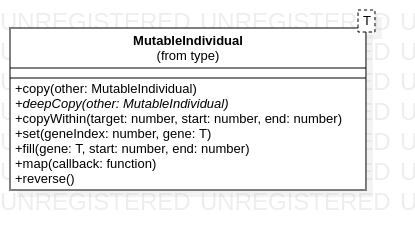
\includegraphics[scale=0.6]{mem/images/cap-4/4.2.2(Individuos)/MutableIndividual.png}
    \caption{Diagrama de clase de \texttt{MutableIndividual}}
    \label{fig:mutableindividual-uml}
\end{figure}

\texttt{MutableIndividual} es una clase también abstracta que hereda de \texttt{BaseIndividual}, y que implementa la interfaz \texttt{Mutable}. Esta interfaz introduce los métodos más comunes para hacer cambios en el contenido del genotipo del array; como por ejemplo el método \texttt{set}, \texttt{fill} o \texttt{map}, los cuales ya están presentes en los arrays de JavaScript. \\

El único método abstracto que presenta esta clase es \texttt{deepCopy}, que seirve para especificar como se haría una copia profunda del genotipo.

\subsubsection{BinaryIndividual}

\begin{figure}[ht]
    \centering
    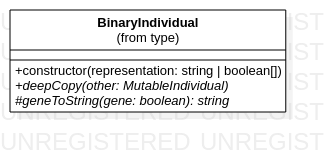
\includegraphics[scale=0.7]{mem/images/cap-4/4.2.2(Individuos)/BinaryIndividual.png}
    \caption{Diagrama de clase de \texttt{BinaryIndividual}}
    \label{fig:binaryindividual-uml}
\end{figure}

El individuo binario (\texttt{BinaryIndividual}), es uno de los más utilizados dentro de los algoritmos evolutivos, y fue la primera representación con la que se construyó un algoritmo genético \cite{holland1992adaptation}. \\

Para implementar este tipo de individuos, se ha extendido de la clase \texttt{MutableIndividual}, pero con el tipo de dato \texttt{boolean}, que es el que contendrá el genotipo.

\subsubsection{NumericIndividual}

\begin{figure}[ht]
    \centering
    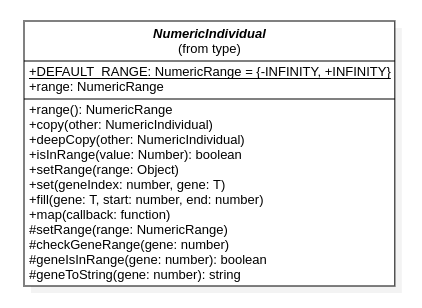
\includegraphics[scale=0.7]{mem/images/cap-4/4.2.2(Individuos)/NumericIndividual.png}
    \caption{Diagrama de clase de \texttt{NumericIndividual}}
    \label{fig:binaryindividual-uml}
\end{figure}

El individuo numérico es una clase abstracta para aglutinar a los individuos que contienen números enteros y flotantes, los cuales tienen la mayoría de métodos comunes a excepción de su representación. \\

Los individuos con codificación numérica contienen una parámetro \texttt{range} que especifica el rango en el que se encuentran los genes de dicho individuo. Para esta librería, los individuos solo podrán tener un rango, que se aplicará a todo los genes o valores del individuo, aunque puede caber la posibilidad de que se tengan varios rangos que se apliquen a los intervalos de genes especificados. \\

Para implementar esta clase, es necesario que se sobrescriban la mayoría de métodos presentes en \texttt{MutableIndividual} para hacer la gestión de errores, garantizando que los valores que se introducen para hacer cambios están dentro del rango permitido.

\subsubsection{IntegerIndividual}

\begin{figure}[ht]
    \centering
    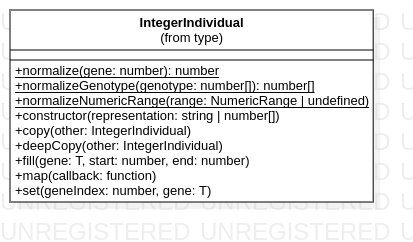
\includegraphics[scale=0.7]{mem/images/cap-4/4.2.2(Individuos)/IntegerIndividual.png}
    \caption{Diagrama de clase de \texttt{IntegerIndividual}}
    \label{fig:binaryindividual-uml}
\end{figure}

El individuo entero es un \texttt{NumericIndividual} que contiene en su genotipo tan solo números enteros, por ello, lo más importante es garantizar que cualquier número que se introduzca en el array sea un número entero. \\

Este criterio se puede garantizar de una manera más restrictiva si se genera un error cada vez que se intente establecer un número flotante como un valor dentro del genotipo, pero en esta implementación se ha optado por redondear siempre los valores numéricos que se intenten introducir, de tal forma se garantiza que estos siempre sean enteros.

\subsubsection{FloatingIndividual}

\begin{figure}[ht]
    \centering
    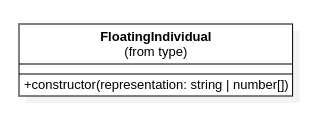
\includegraphics[scale=0.7]{mem/images/cap-4/4.2.2(Individuos)/FloatingIndividual.png}
    \caption{Diagrama de clase de \texttt{FloatingIndividual}}
    \label{fig:binaryindividual-uml}
\end{figure}

Por otra parte, tenemos el individuo numérico que contiene valores en punto flotante. Esta clase es prácticamente idéntica a la clase base de individuos numéricos (\texttt{NumericIndividual}), puesto que tan solo se debe implementar el constructor.

\subsection{Generador de individuos}

Dentro del ciclo de un algoritmo evolutivo, la generación de individuos aleatorios es la fase inicial. En esta sección se expondrá como se ha implementado el generador de individuos aleatorios y las partes que este ha involucrado. \\

Tal y como ocurre en el caso anterior, el generador de individuos aleatorios debe hacerse a medida para el individuo que se pretende generar, y de tal forma que sea extensible para cualquier tipo de individuo a implementar en un futuro. Para \textbf{genetics.js} se han creado un generador aleatorio por cada tipo de individuo que se ha desarrollado, siempre tratando de reutilizar la mayor parte de código estableciendo una jerarquía de herencia.

\begin{figure}[ht]
    \centering
    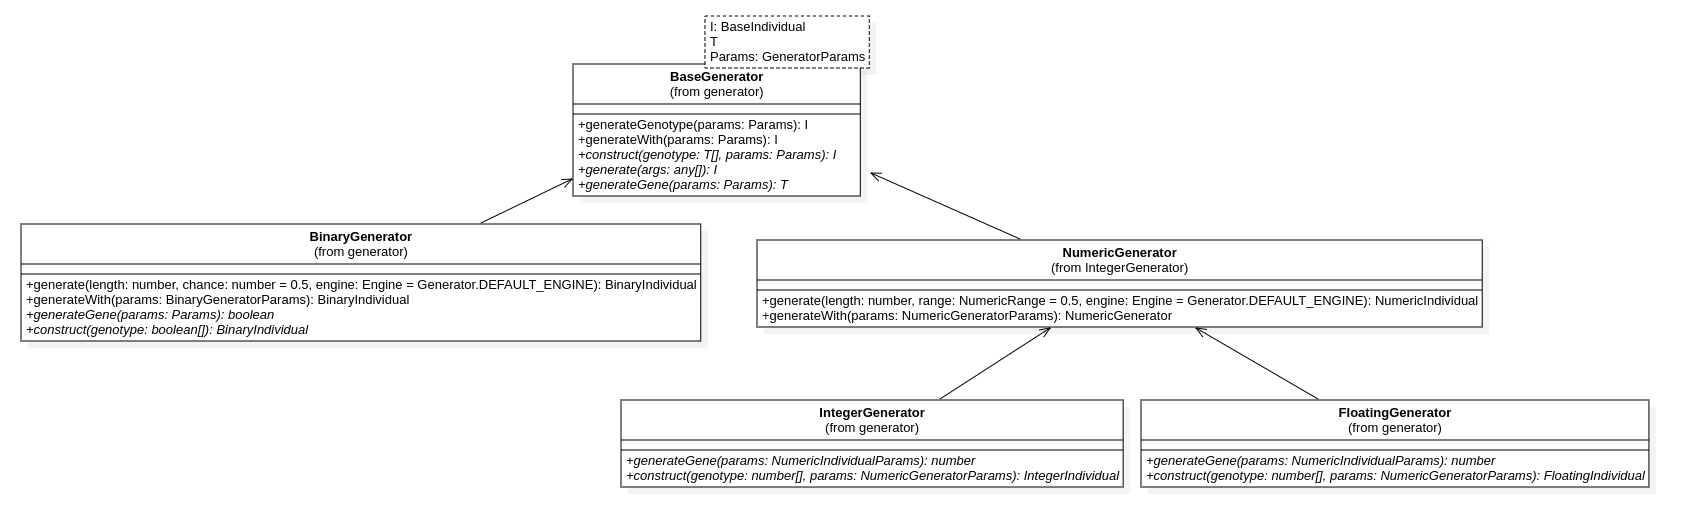
\includegraphics[scale=0.3]{mem/images/cap-4/4.2.3(Generador)/Generator.png}
    \caption{Diagrama de la jergarquía de clases del generador de individuos}
    \label{fig:generator-uml}
\end{figure}

\subsubsection{BaseGenerator e interfaz IndividualGenerator}

\begin{figure}[ht]
    \centering
    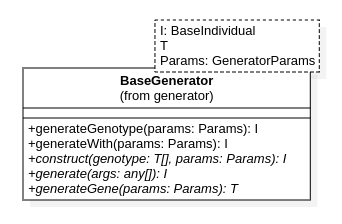
\includegraphics[scale=0.5]{mem/images/cap-4/4.2.3(Generador)/BaseGenerator.png}
    \caption{Diagrama de clase de \texttt{BaseGenerator}}
    \label{fig:generator-uml}
\end{figure}

\texttt{IndividualGenerator} es la interfaz básica que se debe implementar para crear un generador aleatorio de individuos. Esta interfaz es genérica, es decir, que debemos especificar cual será el tipo de individuos que pretendemos generar y además deberemos especificar los parámetros concretos del generador a implementar. \\

Para establecer los parámetros del generador hemos creado otra interfaz (\texttt{GeneratorParams}), la cual de manera básica tiene dos propiedades: 

\begin{itemize}
    \item \texttt{engine}: Es el engine que se utilizara como semilla del generador aleatorio, independientemente del tipo que se quiera generar.
    \item \texttt{length}: Es el tamaño del individuo que se va a generar.
\end{itemize}

Esta interfaz \texttt{GeneratorParams} será también extendida para indicar los parámteros concretos del generador. \\

Para ofrecer una implementación básica de un generador de individuos se ha creado la clase \texttt{BaseGenerator}. Esta clase tiene la mayoría de métodos de la interfaz \texttt{IndividualGenerator} implementados, estableciendo además una serie de métodos abstractos para que las clases heredadas puedan implementarlos y así simplificar la tarea de desarrollo. \\

Estos métodos son los siguientes:

\begin{itemize}
    \item \texttt{construct(genotype: T[], params: Params): I}: Este método sirve para construir un individuo dado un genotipo generado, es útil porque en la clase base no se puede acceder al constructor de los individuos concretos que se generarán.
    \item \texttt{generate(...args: any[]): I}: Este es el método básico que podrá ser llamado desde el exterior para generar un individuo. No tiene definidos los parámetros puesto que estos se deberán especificar para cada uno de los generadores que se implementen concretamente.
    \item \texttt{generateGene(params: Params): T}: Este método servirá para generar un gen del genotipo. Espera recibir una lista de parámetros.
\end{itemize}

\subsubsection{BinaryGenerator y BinaryGeneratorParams}

\begin{figure}[ht]
    \centering
    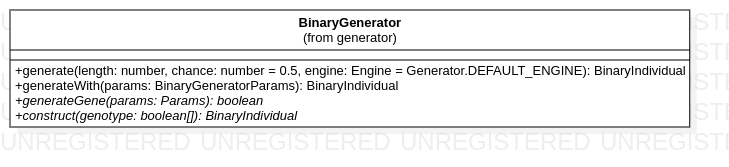
\includegraphics[scale=0.5]{mem/images/cap-4/4.2.3(Generador)/BinaryGenerator.png}
    \caption{Diagrama de clase de \texttt{BinaryGenerator}}
    \label{fig:generator-uml}
\end{figure}

El generador de individuos binarios (\texttt{BinaryGenerator}) tiene bastante importancia en este framework, debido a la gran cantidad de aplicaciones existentes que utilicen individuos binarios como su codificación para las soluciones. \\

Los parámetros de este tipo de generador (\texttt{BinaryGeneratorParams}), son exactamente iguales a los del generador base, pero añadiendo a su vez un campo \texttt{chance} para establecer la probabilidad de que se genere un valor \texttt{true} en el individuo, y de esta manera sesgar el generador.

\subsubsection{NumericGenerator y NumericGeneratorParams}

\begin{figure}[ht]
    \centering
    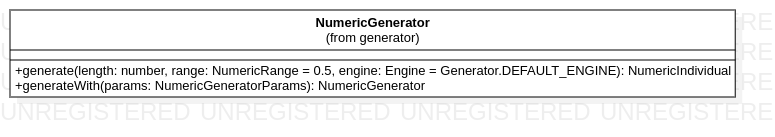
\includegraphics[scale=0.5]{mem/images/cap-4/4.2.3(Generador)/NumericGenerator.png}
    \caption{Diagrama de clase de \texttt{NumericGenerator}}
    \label{fig:generator-uml}
\end{figure}

El generador de individuos numéricos (\texttt{NumericGenerator}) es una clase abstracta que sirve para aglutinar los generadores de individuos numéricos, ya sean de números enteros o reales. \\

La utilidad principal de este generador es especificar los parámetros que tendrá un generador numérico (\texttt{NumericGeneratorParams}), el cual extiende del los parámetros básicos, pero a la vez añade el campo \texttt{range} para especificar el rango que tendrán los genes de los individuos numéricos generados.

\subsubsection{IntegerGenerator y FloatingGenerator}

\begin{figure}[ht]
    \centering
    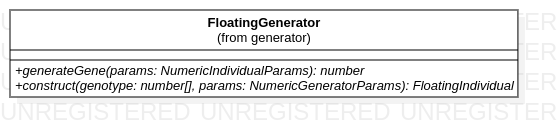
\includegraphics[scale=0.42]{mem/images/cap-4/4.2.3(Generador)/FloatingGenerator.png}
    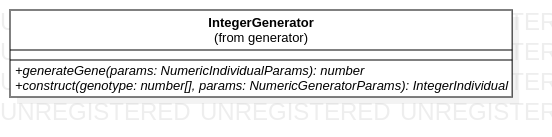
\includegraphics[scale=0.42]{mem/images/cap-4/4.2.3(Generador)/IntegerGenerator.png}
    \caption{Diagrama de clase de \texttt{FloatingGenerator} y \texttt{IntegerGenerator}}
    \label{fig:generator-uml}
\end{figure}

Una vez se ha desarrollado \texttt{NumericGenerator} como generador numérico fundamental, es bastante sencillo extender las clases para generar individuos de números enteros (\texttt{IntegerGenerator}) y de números en punto floatante (\texttt{FloatingGenerator}). \\

Para ello, tan solo se debe implementar el método abstracto \texttt{generateGene}, creando un individuo numérico o un individuo en punto flotante respectivamente. Cabe destacar que los parámetros no varian respecto a aquellos establecidos en \texttt{NumericGeneratorParams}, pues en ambos casos tan solo es necesario especificar el rango como elemento generador.

\subsection{Gestión de la población}

La gestión de la población de individuos es un elemento fundamental para la ejecución de algoritmos evolutivos. Para este propósito, se ha creado una clase \texttt{Ppulation}, que es la encargada de contener el conjunto de individuos de la población, además de proveer de métodos para acceder, modificar o evaluar a dichos individuos. \\

\begin{figure}[ht]
    \centering
    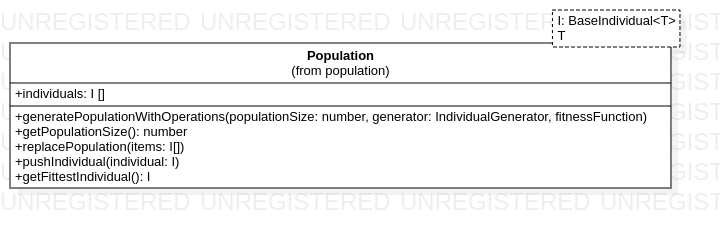
\includegraphics[scale=0.6]{mem/images/cap-4/4.2.4(Population)/Population.png}
    \caption{Diagrama de clase de \texttt{Population}}
    \label{fig:generator-uml}
\end{figure}


Los métodos que contiene esta clase son:

\begin{itemize}
    \item \texttt{generatePopulationWithOperations}: Este método recibe un generador de individuos con sus parámetros, además de una función de fitness y crea a la población de individuos, además de evaluar cual es su fitness.
    \item \texttt{getPopulationSize}: Devuelve el tamaño de la población.
    \item \texttt{replacePopulation}: remplaza los items de la población actual por otros.
    \item \texttt{pushIndividual}: Añade un individuo a la población.
    \item \texttt{getFittestIndividual}: devuelve el individuo que tenga una mayor evaluación en la función de fitness.
    \item \texttt{getPopulationItems}: devuelve los items de la población en forma de \texttt{array}.
\end{itemize}

Ádemás, cabe destacar que esta clase contendrá una serie de estadísticas comunes que se pueden utilizar para visualizar cuales son las métricas que está siguiendo la población en las sucesivas generaciones del algoritmo. Las estadísticas que se pueden consultar serían las siguientes:

\begin{itemize}
    \item \texttt{averageAge}: la edad media de los individuos de la población.
    \item \texttt{averageFitness}: el fitness medio de los individuos de la población.
    \item \texttt{fitnessSum}: la suma total de fitness de los individuos.
    \item \texttt{fittestIndividualIndex}: el índice del individuo con mayor fitness de la población.
\end{itemize}

\subsection{Selección de padres}

La selección de padres es la fase del algoritmo que se corresponde con la elección de aquellos individuos que reproducirán, generando descendencia en la siguiente generación. El criterio de selección de estos individuos puede ser muy variado, pero normalmente es proporcional a cuanto de adaptados al medio estén, lo que se conoce como \textbf{fitness proportional selection}.

Para esta librería se ha desarrollado una selección proporcional al fitness cuya implementación se puede hacer mediante dos métodos diferentes.

\subsubsection{RouletteWheel}

\begin{figure}[ht]
    \centering
    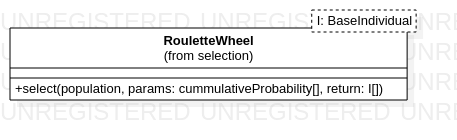
\includegraphics[scale=0.6]{mem/images/cap-4/4.2.5(Selection)/RouletteWheel.png}
    \caption{Diagrama de clase de \texttt{RouletteWheel}}
    \label{fig:generator-uml}
\end{figure}


La idea que se encuentra tras la selección mediante \textit{Roulette Wheel}, es seleccionar a los padres mejor adaptados, pero a su vez dejar un posibilidad a los individuos con una evaluación de fitness peor la posibilidad de ser padres en la siguiente generación. \\

Para simular esta idea se utiliza una ruleta que tiene todos los individuos representados, pero con un área proporcional a su fitness. Al girar esa ruleta, es más probable que se elijan a los individuos mejor adaptados, puesto que su área de selección es mayor, sin embargo, tampoco se impide la selección de indivviduos mucho meńos adaptados, porque aunque su área sea menor, aun tienen una posibilidad de ser seleccionados. Esto nos permite garantizar la variedad en la población seleccionada para evitar que las búsquedas puedan quedar atrapadas en un óptimo local. \\

En la implementación de \textbf{genetics.js}, se espera como parámetros una población, además de un \textit{array} con la probabilidad de selección acumulada normalizada. Tal y como comentamos, esta probabilidad de selección dependerá de la evaluación del fitness del individuo.

\subsubsection{StochasticUniversalSampling}

\begin{figure}[ht]
    \centering
    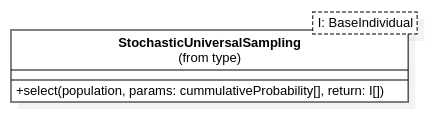
\includegraphics[scale=0.6]{mem/images/cap-4/4.2.5(Selection)/SUS.png}
    \caption{Diagrama de clase de \texttt{StochasticUniversalSampling}}
    \label{fig:generator-uml}
\end{figure}


La otra posibilidad de implemnentación se conoce como \textit{Stochastic Universal Sampling}. La idea es similar a \textit{Roulette Wheel}, pues utiliza también la ruleta proporcional como idea fundamental. Sin embargo, en este método la ruleta no se hace girar tantas veces como individuos se quiera seleccionar, sino que se hace una sola tirada en la que se seleccionan todos los individuos a la vez. Sería el equivalente a una ruleta en la que existieran tantos puntos de selección como individuos, y en una sola tirada se decidieran todos. \\

Los parámetros de este tipo de selección son iguales que en \textit{RouletteWheel}, por tanto es necesario especificar un \texttt{array} con las probabilidades normalizadas acumuladas.

\subsection{Operaciones de cruce}

\begin{figure}[ht]
    \centering
    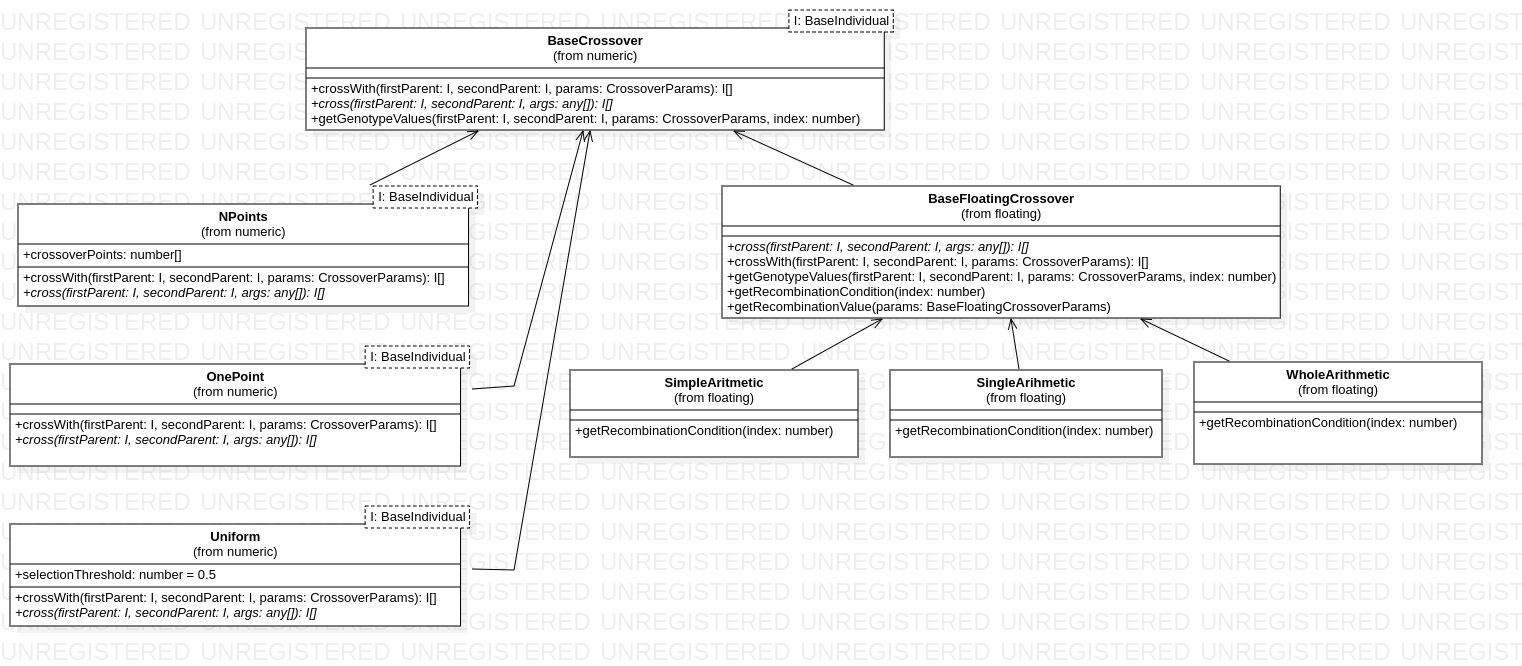
\includegraphics[scale=0.2]{mem/images/cap-4/4.2.6(Crossover)/Crossover.png}
    \caption{Diagrama de clase de las operaciones de cruce}
    \label{fig:my_label}
\end{figure}

Las operaciones de cruce son aquellas que se aplican entre los padres que han sido seleccionados, para así generar una descendencia. Los métodos de cruce entre individuos pueden ser muy diversos, y dependen normalmente del tipo de individuos a los que se les esté aplicando la operación de cruce.\\

Para implementar los operadores de cruce, hemos utilizado una jerarquía de herencia que se implementa a partir de una interfaz, a partir de la cual hemos desarrollado los métodos de cruce más comunes.


\subsubsection{BaseCrossover e interfaz Crossover}

\begin{figure}[ht]
    \centering
    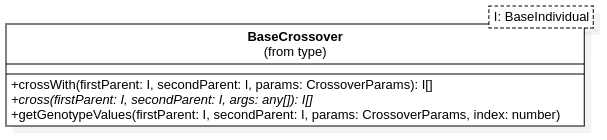
\includegraphics[scale=0.5]{mem/images/cap-4/4.2.6(Crossover)/BaseCrossover.png}
    \caption{Diagrama de clase de \texttt{BaseCrossover}}
    \label{fig:my_label}
\end{figure}

En las operaciones de cruce que hemos considerado, se seleccionan dos individos como padres, y a partir de ellos, aplicando la operación correspondiente, se generan dos hijos como descendencia. Siguiendo la metodología utillizada previamente, lo que haremos será elaborar una interfaz (\texttt{Crossover}), en la que se definan los métodos que deberán tener todas las operaciones de cruce.

\begin{itemize}
    \item \texttt{crossWith(firstParent: I, secondParent: I, params: Params): I[]}: Este método sirve para llevar a cabo las operaciones de crossover mediante los parámetros establecidos para cada uno de los métodos.
    \item \texttt{cross(firstParent: I, secondParent: I, ...args: any[]): I[]}: Este método sirve para llamar a la operación de cruce con dos padres y con los argumentos variables que se hayan decidido para cada método concreto. Sirve para ofrecer una llamada más amigable para la función, en lugar de pasar un objeto de parámetros.
\end{itemize}

Además de estos métodos, se ha includido una interfaz de parámetros básicos para estas operaciones (\texttt{CrossoverParams}), estos parámetros incluyen dos elementos de manera genérica:

\begin{itemize}
    \item \texttt{engine}: Es el engine que se utilizará para el generador aleatorio.
    \item \texttt{individualConstructor}: Los operadores de cruce necesitan construir los individuos que conformarán la descendencia. Es por ello que un parámetro necesario para la operación de cruce es el constructor de los individos. Pasar este tipo de funciones como parámetro es una de las ventajas de usar un lenguaje como TypeScript.
\end{itemize}

A partir de la interfaz \texttt{Crossover} y los parámetros \texttt{CrossoverParams}, se ha construido una clase base abstracta (\texttt{BaseCrossover}). Esta clase contiene una implementación básica de una operación de cruce, de tal forma que facilita la tarea a la hora de llevar a cabo la extensión e implementación de nuestras propias operaciones. \\

El único método abstracto que posee esta clase y que se puede implementar es el siguiente:

\begin{itemize}
    \item \texttt{getGenotypeValues(firstParent: I, secondParent: I, index: number)}: Este método se utiliza para obtener el valor del genotipo de la descendencia dado un índice concreto.
\end{itemize}

\subsubsection{NPointsCrossover}

\begin{figure}[ht]
    \centering
    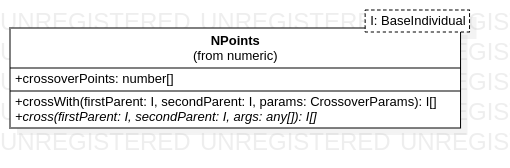
\includegraphics[scale=0.5]{mem/images/cap-4/4.2.6(Crossover)/NPoints.png}
    \caption{Diagrama de clase de \texttt{NPointsCrossover}}
    \label{fig:my_label}
\end{figure}

El crossover por n puntos (\texttt{NPointsCrossover}), es uno de los tipos de crossover más famosos. Su procedimiento consiste en elegir dos padres, y elegir n puntos de cruce entre ellos aleatoriamente. Cada uno de los dos individuos de la descendencia se formará escogiendo de manera correlativa los genes de los padres. \\

Para nuestra implementación, se ha creado la clase \texttt{NPointsCrossover} que extiende de \texttt{BaseCrossover} y que tiene impleemntado el método \texttt{getGenotypeValues}, cuyo objetivo es decidir de cual de cada uno de los padres elige el material genético, teniendo en cuenta que se debe hacer de manera alternativa.

A su vez, también se ha creado la interfaz \texttt{NPointsCrossoverParams}, esta interfaz sirve para especificar los parámetros de esta operación, extendiendo de \texttt{CrossoverParams}. El único parámetro adicional que se ha añadido ha sido:

\begin{itemize}
    \item \texttt{numberOfCrossoverPoints}: es el número de puntos de cruce elegidos para llevar a cabo la operación.
\end{itemize}

\subsubsection{OnePointCrossover}

\begin{figure}[ht]
    \centering
    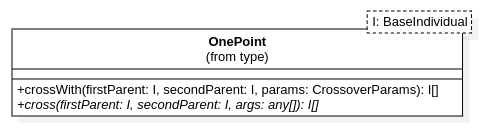
\includegraphics[scale=0.5]{mem/images/cap-4/4.2.6(Crossover)/OnePoint.png}
    \caption{Diagrama de clase de \texttt{OnePointCrossover}}
    \label{fig:my_label}
\end{figure}

El crossover de un solo punto es un caso concreto de el crossover de n puntos para $n = 1$. La implementación de este método es bastante sencilla una vez hecho el crossover de n puntos, puesto que tan solo habría que llamar a este método con \texttt{numberOfCrossoverPoints: 1}. Además, cabe destacar que este tipo de operación no tiene ningún parámetro adicional.

\subsubsection{UniformCrossover}

\begin{figure}[ht]
    \centering
    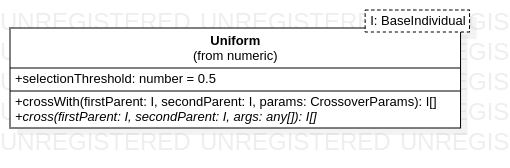
\includegraphics[scale=0.5]{mem/images/cap-4/4.2.6(Crossover)/Uniform.png}
    \caption{Diagrama de clase de \texttt{UniformCrossover}}
    \label{fig:my_label}
\end{figure}

El crossover uniforme consiste en escoger de cuales de los dos padres se escoge el material genético en función de un valor aleatorio de probabilidad que se genera por cada gen, comparándolo con un valor umbral dado como parámetro. Este método de recombinación permite hacer variaciones más importantes en los cromosomas de la descendencia. \\

Para la implementación de este método se ha creado la clase \texttt{UniformCrossover} que extiende de \texttt{BaseCrossover}, además de la interfaz \texttt{UniformCrossoverParams} que extiende de \texttt{CrossoverParams} y que tiene como parámetro el umbral que se utilizará para determinar de cual de los padres se obtiene el material genético para la descendencia.

\subsubsection{BaseFloatingCrossover}

\begin{figure}[ht]
    \centering
    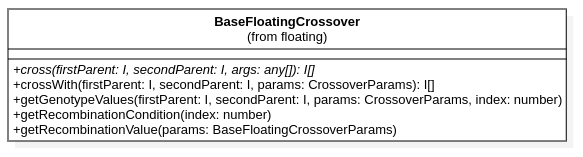
\includegraphics[scale=0.5]{mem/images/cap-4/4.2.6(Crossover)/BaseFloating.png}
    \caption{Diagrama de clase de \texttt{BaseFloatingCrossover}}
    \label{fig:my_label}
\end{figure}

Mientras que los tres tipos de operaciones de cruce descritos anteriormente pueden aplicarse a cualquier tipo de individuos, existen métodos que solo pueden aplicarse a individuos concretos. Es el caso de los métodos siguientes, que solo serán aplicados a individuos de punto flotante. \\

Para aglutinar los métodos de crossover de individuos flotantes se ha creado la clase abstracta \texttt{BaseFloatingCrossover}. Esta clase, tiene implementado el método \texttt{getGenotypesValue}, de tal forma que en función de una condición que se implementará de manera concreta en las clases heredadas, se devolverá el valor del genotipo como: 

\begin{equation}
    z^x_i = \alpha x_i + (1 - \alpha)y_i
\end{equation}

\begin{equation}
    z^y_i = \alpha y_i + (1 - \alpha)x_i
\end{equation}

Donde $x$ e $y$ son los padres elegidos en la operación de recombinación y $z^x$ y $z^y$ son los individuos $x$ e $y$ de la descendencia respectivamente. Todos ellos están evaluados en su gen $i$, es decir en el $i$-esimo valor de su genotipo. \\

Tal y como podemos comprobar, esta operación depende de un parámetro $\alpha$, que debe ser pasaod como parámetro en la interfaz \texttt{BaseFloatingCrossoverParams} que exiende de \texttt{CrossoverParams}.

\subsubsection{SimpleArithmeticRecombination}

\begin{figure}[ht]
    \centering
    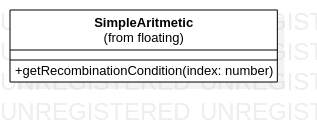
\includegraphics[scale=0.7]{mem/images/cap-4/4.2.6(Crossover)/SimpleArithmetic.png}
    \caption{Diagrama de clase de \texttt{SimpleArithmeticRecombination}}
    \label{fig:my_label}
\end{figure}


Este es uno de los tres tipos de recombinación que se han implementado para individuos de punto flotante. Esta recombinación consiste en hacer la mezcla entre los valores de los genotipos de los padres seleccionados en función de si el índice del elemento del genotipo que se quiere obtener es menor que un cierto índice $k$ generado aleatoriamente. \\

La expresión que se utilizaría para definir a la descendencia sería:

\begin{equation}
    <x_1, \dots, x_k, \alpha \cdot y_{k+1} + (1 - \alpha) \cdot x_{k+1}, \dots, \alpha \cdot y_n + (1 - \alpha) \cdot x_n >
\end{equation}

\begin{equation}
    <y_1, \dots, y_k, \alpha \cdot x_{k+1} + (1 - \alpha) \cdot y_{k+1}, \dots, \alpha \cdot x_n + (1 - \alpha) \cdot y_n >
\end{equation}

Como vemos, este método de recmobinación depende también de un parámetro $\alpha$. 

La implementación de este método se ha hecho mediante la clase \texttt{SimpleArithmeticRecombination}, con la interfaz de parámetros \texttt{BaseFloatingCrossoverParams}, en la que ya viene especificado el parametro $\alpha$.

\subsubsection{SingleArithmeticRecombination}

\begin{figure}[ht]
    \centering
    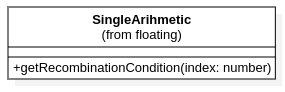
\includegraphics[scale=0.7]{mem/images/cap-4/4.2.6(Crossover)/SingleArithmetic.png}
    \caption{Diagrama de clase de \texttt{SingleArithmeticRecombination}}
    \label{fig:my_label}
\end{figure}


Esta operación destaca por producir pocos cambios en la descendencia respecto a los padres, pues tan solo se aplicará la expresión de mezcla de genotipos en una sola posición $k$ elegida de manera aleatoria. \\

La expresión que repesenta este método es la siguiente:

\begin{equation}
    <x_1, \cdots ,x_{k−1}, \alpha \cdot y_k + (1 - \alpha) \cdot x_k, x_{k+1}, \cdots ,x_n >
\end{equation}
\begin{equation}
    <y_1, \cdots ,y_{k−1}, \alpha \cdot x_k + (1 - \alpha) \cdot y_k, y_{k+1}, \cdots ,y_n >
\end{equation}

Para su implementación se ha creado la clase \texttt{SingleArtihmeticRecombination}, con la interfaz de parámetros \texttt{BaseFloatingCrossoverParams}.

\subsubsection{WholeArithmeticRecombination}

\begin{figure}[ht]
    \centering
    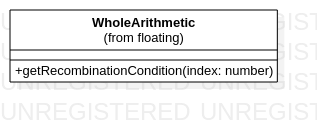
\includegraphics[scale=0.7]{mem/images/cap-4/4.2.6(Crossover)/WholeArithmetic.png}
    \caption{Diagrama de clase de \texttt{WholeArithmeticRecombination}}
    \label{fig:my_label}
\end{figure}

Este es el último tipo de recombinación para individuos de números en punto flotante. Se caracteriza por provocar un cambio bastante drástico en el genotipo de la descendencia respecto al genotipo de los padres, pues aplica la expresión de mezcla de genotipos en todos los genes de los individuos generados. \\

La expresión que lo caracteriza es la siguiente:

\begin{equation}
    z^x = \overline{x} + (1 - \alpha) \cdot \overline{y}
\end{equation}

\begin{equation}
    z^y = \overline{y} + (1 - \alpha) \cdot \overline{x}
\end{equation}

La implementación de este método se ha hecho mediante la clase \texttt{WholeArithmeticRecombination}.

\subsection{Mutaciones}

\begin{figure}[ht]
    \centering
    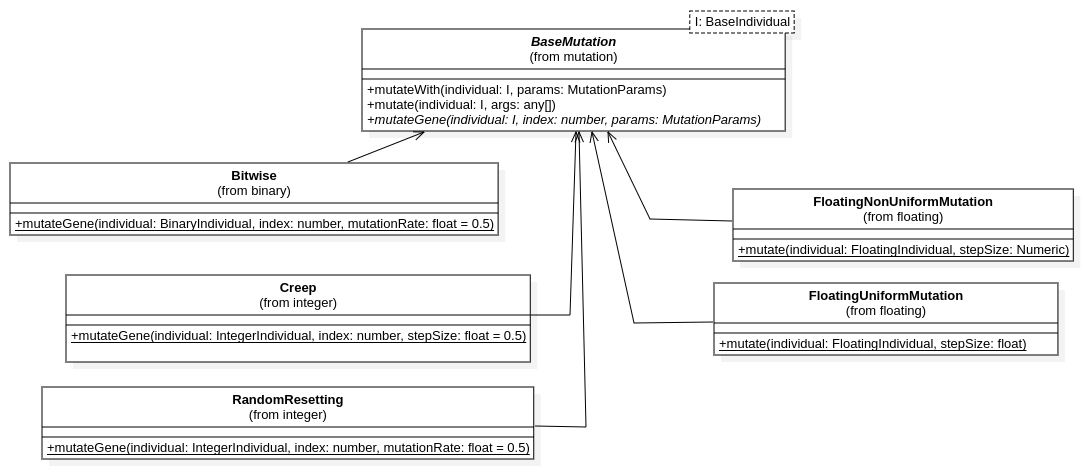
\includegraphics[scale=0.3]{mem/images/cap-4/4.2.7(Mutation)/Mutation.png}
    \caption{Diagrama de clase para los operadores de mutación }
    \label{fig:my_label}
\end{figure}

Las operaciones de mutación sirven para aplicar un cierto grado de aleatoriedad a los individuos generados como descendencia después de aplicar una operación de recombinación. \\

Dentro de los algoritmos evolutivos, este tipo de operaciones son las que incrementan el grado de diversidad existente en las soluciones obtenidas a partir de la recombinación, por ello se aplica a la descendencia obtenida. \\

Para su implementación se ha seguido el mismo patrón que con la recombinación, es decir, crear una jerarquía de clases que se implemente a partir de una interfaz báse.

\subsubsection{MutationBase e interfaz Mutation}

\begin{figure}[ht]
    \centering
    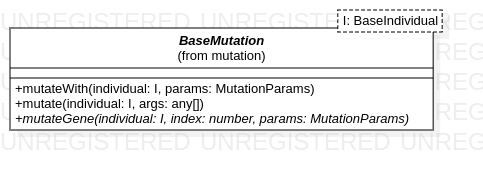
\includegraphics[scale=0.4]{mem/images/cap-4/4.2.7(Mutation)/BaseMutation.png}
    \caption{Diagrama de clase de \texttt{BaseMutation}}
    \label{fig:my_label}
\end{figure}

Para definir las operaciones de mutación que hemos implementado, se ha creado la interfaz \texttt{Mutation}, la cual cuenta con dos métodos, que deben ser implementados para crear la operación deseada.

\begin{itemize}
    \item \texttt{mutateWith(individual: I, params: Params): void}: Este método sirve para aplicar una mutación sobre el individuo que se pasa como parámetro con los parámetros que se indican.
    \item \texttt{mutate(individual: I, ...args: any[]): void}: Este método sirve también para aplicar la mutación sobre el individuo que se pasa como parámetro, sin embargo, sirve para especificar los parámetros de la mutación de manera más cómoda.
\end{itemize}

Al igual que ocurre con las operaciones de cruce, en la mutación también debemos definir los parámetros con los cuales se aplicará. Para ello, hemos definido la clase genérica \texttt{MutationParams}, la cual tiene un solo componente:

\begin{itemize}
    \item \texttt{engine}: El engine que se utilizará para el generador aleatorio.
\end{itemize}

A partir de la interfaz \texttt{Mutation} y con los parámetros \texttt{MutationParams}, se ha creado una clase base abstracta (\texttt{MutationBase}) que implementa la mayoría de métodos utilizados para llevar a cabo operaciones de mutación.\\

Esta clase posee una serie de métodos abstractos que se deben implementar para extenderla y facilitar así la tarea de desarrollar nuestros propios métodos de mutación.

\begin{itemize}
    \item \texttt{mutate(individual: I, ...args: any[]): void}: Este método heredado de la interfaz \texttt{Mutable} no se ha implementado, pues los parámetros concretos dependen del método de mutación.
    \item \texttt{mutateGene(individual: I, index: number, params: Params): void}: Este método abstracto será utilizado para mutar el gen especificado por el índice.
\end{itemize}

\subsubsection{BitwiseMutation}

\begin{figure}[ht]
    \centering
    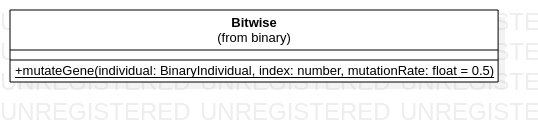
\includegraphics[scale=0.4]{mem/images/cap-4/4.2.7(Mutation)/Bitwise.png}
    \caption{Diagrama de clase de \texttt{BitwiseMutation}}
    \label{fig:my_label}
\end{figure}

Esta mutación se aplica a individuos binarios (\texttt{BinaryIndividual}) y es muy común en muchos algoritmos evolutivos. Consiste en intercambiar los bits del individuo, verdadero por falso y viceversa, en función de un parámetro que se conoce como la tasa de mutación (\textit{mutation rate}). \\

Para implementar este método de mutación se ha creado la clase \texttt{BitwiseMutation}. Además se ha utilizado la interfaz \texttt{BitwiseMutationParams}, que extiende \texttt{MutationParams} y que incluye un miembro \texttt{mutationRate}, que especifica la probabilidad que tiene cada gen de ser mutado.

\subsubsection{CreepMutation}

\begin{figure}[ht]
    \centering
    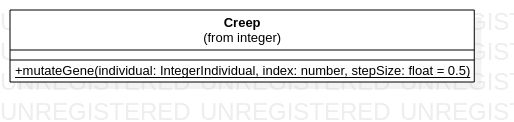
\includegraphics[scale=0.4]{mem/images/cap-4/4.2.7(Mutation)/CreepMutatioon.png}
    \caption{Diagrama de clase de \texttt{CreepMutation}}
    \label{fig:my_label}
\end{figure}

El siguiente tipo de mutación se aplica a individuos de tipo entero (\texttt{IntegerIndividual}), y consiste en mutar cada uno de los genes del individuo añadiendo una cantidad $\delta$ al valor del gen, obtenida a partir de una distribución normal de probabilidad y redondeado para devolver un número entero. \\

Esta distribución de probabilidad tiene como parámetros $\mu = 0$ y $\sigma$, donde el último se corresponde al \textit{step size} o tamaño en el que se quiere variar el gen:

\begin{equation}
    x_i = x_i + |\mathcal{N}(0, \sigma)|
\end{equation}

Para implementar este método de mutación se ha utilizado la clase \texttt{CreepMutation}, y la interfaz \texttt{CreepMutationParams}, la cual tiene especificado el \texttt{stepSize} que se desea como parámetro.

\subsubsection{RandomResetting}

\begin{figure}[ht]
    \centering
    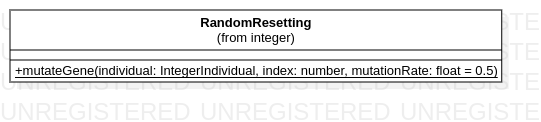
\includegraphics[scale=0.4]{mem/images/cap-4/4.2.7(Mutation)/RandomResetting.png}
    \caption{Diagrama de clase de \texttt{RandomResetting}}
    \label{fig:my_label}
\end{figure}

La operación de \textit{random resetting} sería el equivalente al \textit{bitwise mutation} para individuos enteros (\texttt{IntegerIndividual}). En este tipo de mutación, se elige de manera uniforme un número al azar entre el rango de valores permitidos, el cual se establecerá como el nuevo valor del gen mutado.

Para implementar este método se ha utilizado la clase \texttt{RandomResetting} la cual no tiene parámetros, puesto que el rango permitido de valores es elegido desde el propio individuo que se quiere mutar.

\subsubsection{FloatingNonUniformMutation}

\begin{figure}[ht]
    \centering
    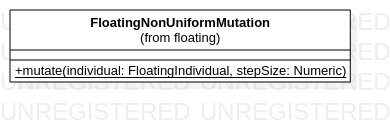
\includegraphics[scale=0.4]{mem/images/cap-4/4.2.7(Mutation)/FloatingNonUniformMutation.png}
    \caption{Diagrama de clase de \texttt{FloatingNonUniform}}
    \label{fig:my_label}
\end{figure}

Esta mutación es similar a \textit{Creep mutation} pero para individuos en punto flotante (\texttt{FloatingIndividual}). A partir de una distribución normal de probabilidad se ha obtenido un número flotante que se añade al valor del gen, haciendo que se produzca una variación del mismo.

\begin{equation}
    x_i = x_i + \mathcal{N}(0, \sigma)
\end{equation}

La distribución normal de probabilidad tiene dos parámetros ($\mu$ y $\sigma$), pero al igual que en \textit{Creep mutation}, se establece el valor $\mu = 0$ y a $\sigma$ se le denomina \textit{step size}, siendo la variable que controla la cantidad de variación que se aplicará a los genes. \\

Para la impelemntación de este método se ha creado la clase \texttt{FloatingNonUniformMutation}, y la interfaz de parámetros \texttt{FloatingNonUniformMutationParams} que contiene un único parámetro y es el \texttt{stepSize} que se le aplicará a la operación.

\subsubsection{FloatingUniformMutation}

\begin{figure}[ht]
    \centering
    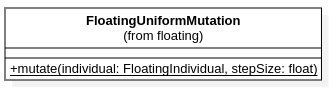
\includegraphics[scale=0.4]{mem/images/cap-4/4.2.7(Mutation)/FloatingUniformMutation.png}
    \caption{Diagrama de clase de \texttt{FloatingUniform}}
    \label{fig:my_label}
\end{figure}

De manera equivalente a como ocurre en el caso de individuos de números enteros, también existe un equivalente al \texttt{BitwiseMutation} para números en punto flotante y es la mutación uniforme. Esta mutación consiste en sustituir el gen mutado por un valor seleccionado de manera uniforme en el rango de valores permitidos. \\

La implementación de este método se lleva a cabo mediante la clase \texttt{FloatingUniformMutation}, que al igual que en \texttt{RandomResetting} no tiene parñametros adicionales puesto que el rango de valores es un atributo del individuo que se desea mutar.

\subsection{Reemplazo}

El reemplazo de los individuos es la fase que sigue una vez se ha generado la descendencia a partir de la población que se encontraba inicialmente en la generación. \\

Una vez que se ha generado esa descendencia tendremos una cantidad de individuos perteneciente a la población inicial y otra cantidad de individuos perteneciente a la descendencia, el proceso de selección se encargará de discernir cuales dentro de todos estos individuos serán los que pasen a la siguiente generación. \\

En la implementación de esta librería, hemos considerado que el tamaño de la población y descendencia es igual. Por tanto si definimos $\lambda$ como el tamaño de la población, el tamaño de la descendencia y de la población se considera $\lambda + \lambda$, y de este tamaño debemos elegir tan solo $\lambda$ siguiendo algún criterio.

\begin{equation}
    \lambda + \lambda \rightarrow \lambda
\end{equation}

Los métodos de reemplazo que se han implementado han sido los siguientes:

\subsubsection{AgeBasedReplacement}

Este método de remplazo consiste en seleccionar a los individuos mas jóvenes de entre la población y la descendencia. En nuestro caso, en el que los tamaños de la población y la descendencia coinciden, esta operación se corresponderá a seleccionar tan solo a los individuos de la descendencia. \\

La principal ventaja de este método de selección es la eficiencia, pues a la hora de tener poblaciones de una gran cantidad de individuos tan solo deberían devolverse los individuos de la nueva población. \\

Para implementarlo se ha utilizado la clase \texttt{AgeBasedReplacement}, la cual tiene un único método \texttt{replace} que tiene como parámetros la población inicial y el offspring, a partir de los cuales se quiere generar la población de remplazo.

\subsubsection{FitnessBasedReplacement}

El criterio que se sigue para llevar a cabo el remplazo mediante este método es el fitness que posee el individuo. De esta forma, cuando se tiene la población inicial y la descendencia, los individuos de ambas se deben ordenar de acuerdo a su fitness, seleccionando solo los mejores. \\

Este método es bastante elitista, es decir que tan solo elige a los mejores de la población y la descendencia. Esto hace que se conserven los individuos mejores adaptados durante más generaciones. Sin embargo, también conlleva una pérdida de diversidad en los individuos y un aumento en la complejidad de la envaluación en poblaciones de un gran tamaño. \\

La implementación se ha hecho mediante la clase \texttt{FitnessBasedReplacement}, la cual tiene un método replace, que recibe la población inicial y la descendencia, al igual que en el caso anterior.

\subsection{Fitness}

La función de fitness se utiliza para evaluar cuanto de adaptado se encuentra un individuo al entorno. Si estamos hablando de un problema de optimización combinatoria, esta función se corresponde con la que queremos optimizar. En esta librería, la función de fitness se trata de maximizar, de tal forma que se consideran mejores las funciones de fitness con valores más altos.\\

La implementación de la función de fitness ha sido bastante simple, de tal foma que solo se ha establecido el esquema de la función como un tipo.

\begin{center}
    \texttt{(individual: I, ...args: any[]) => number}
\end{center}

Como podemos ver es una función que recibe como parámetros el individuo que se quiere evaluar además de cualquier parámetro adicional. De esta forma dependiendo de la aplicación concreta para la cual queramos utilizar esta librería, se debera implementar esta función de manera concreta.

\subsection{Condición de finalización}

La condición de finalización es la que indica cuando la ejecución del algoritmo evolutivo ha terminado. Este criterio de finalización se suele establecer en función del estado de la población en el momento concreto de la ejecución. \\

En el caso de \textbf{genetics.js}, la condición de parada que se ha logrado implementar es la de llegar a un número concreto de generaciones, es decir que el algoritmo se pare cuando se hayan ejecutado una serie de generaciones que se establecen como parámetro. \\

Esto se hace mediante la clase \texttt{MaxGenerations}, que recibe como parámetro el número máximo de generaciones que queremos que se ejecuten.